%% MADKE-X manuscript — Elsevier elsarticle template.
%% Faithful reproduction of the current draft (Extra_Files/MADKE-X.pdf); revisions are applied step by step.
%% Compile: pdflatex -> bibtex -> pdflatex -> pdflatex (VS Code LaTeX Workshop does this on save;
%% Overleaf does it automatically).
\documentclass[preprint,12pt]{elsarticle}

\usepackage{lmodern}
\usepackage{amsmath,amssymb}
\usepackage{graphicx}
\usepackage{booktabs}
\usepackage{multirow}
\usepackage{array}
\usepackage{xcolor}
\usepackage[ruled,vlined,linesnumbered]{algorithm2e}
\usepackage{siunitx}
\usepackage[hidelinks]{hyperref}

\graphicspath{{figures/}}
\SetKwInOut{Input}{Input}
\SetKwInOut{Output}{Output}

%% Shorthands
\newcommand{\madke}{MADKE}
\newcommand{\madkex}{MADKE-X}

\journal{Expert Systems with Applications}

\begin{document}

\begin{frontmatter}

\title{MADKE-X: Traceable, Evidence-Governed Multi-Agent Debate for Knowledge-Intensive Question Answering}

\author[iu]{Muhammad Ali}
\author[iu]{Muhammad Talha}
\affiliation[iu]{organization={Department of Computer Science, Iqra University, Airport Campus},
            city={Karachi},
            country={Pakistan}}

\begin{abstract}
Multi-agent debate lets several large language model (LLM) agents argue towards an answer, and MADKE (Wang et al., \emph{Neurocomputing}, 2025) improves it with a shared evidence pool, per-agent evidence selection, a consistency judge and a summariser. A prior audit of the public release identified 20 problems: eight implementation defects (for example, the summariser receives the question and the debate in swapped slots, and 59 of 500 test questions are silently skipped), poorly ordered and redundant evidence pools, under-powered reporting, and answers that carry no trace of the evidence behind them. We propose MADKE-X, an expert-system-style refinement of MADKE that keeps its control flow and prompts but adds four components: a failure-aware interface layer, an evidence governor (paper-sized pool, de-duplication, reciprocal-rank-fusion ordering), a decision trace with $\{E\#\}$ citations and a lexical support check, and a bounded verification step triggered by the support check. We evaluate MADKE-X against MADKE in two ways. Executed offline, with the unmodified original and the patched code driven by identical scripted agents on the shipped data (not altered; SHA-256 verified), MADKE-X satisfies every invariant that MADKE violates: summariser prompt correct 100\% versus 0\%, evidence delivered as selected 100\% versus 16\%, debate stopped at the round of agreement 100\% versus 78\%, and 500 versus 441 of 500 questions processed. Its evidence ordering puts an answer-bearing passage among the first three for 76.0\% versus 51.6\% (TriviaQA), 66.4\% versus 60.4\% (NQ), 40.0\% versus 21.5\% (HotpotQA) and 25.0\% versus 11.5\% (2WikiMultihopQA) of questions (paired exact McNemar $p\le 0.01$), and its paper-sized pool cuts the evidence listing sent to every agent call by 45.0\% (estimated), at a cost of about 0.68\,ms per question for the ordering. Second, we give a complete, pre-specified end-to-end protocol that mirrors the evaluation of MADKE (the five shipped datasets, five baselines plus MADKE re-run, three backbones, F1/EM/GPT-4 score/Cons/Co2, ablation, sensitivity, token cost, case study); because no LLM access was available, the accuracy cells are left empty and are not estimated. MADKE-X therefore establishes correctness, traceability and cost, and leaves its accuracy effect to be measured.
\end{abstract}


\begin{keyword}
multi-agent debate \sep large language models \sep retrieval-augmented generation \sep
explainable agentic AI \sep evidence attribution \sep question answering
\end{keyword}

\end{frontmatter}

\section{Introduction}
\label{sec:introduction}

Large language models (LLMs) answer knowledge-intensive questions less reliably than their fluency suggests, and a standard remedy is to give several model instances the same question and let them critique each other \cite{du2024debate,liang2024divergent,smit2024mad}. MADKE \cite{wang2025madke} adds external knowledge to this debate: a shared pool of Wikipedia and web passages from which each agent selects at most three items per round, a judge that stops the debate when the agents agree, and a summariser that writes the final answer. It is reported to outperform single-agent prompting, chain-of-thought \cite{wei2022cot}, self-consistency \cite{wang2023sc}, retrieval-augmented generation \cite{lewis2020rag} and plain debate on five benchmarks.

An audit of the released implementation \cite{ali2026audit} showed that the published pipeline does not behave as described and offers no way to see why it produced an answer. A first set of repairs and their offline proofs was reported separately (Part~II). This paper turns them into one method, MADKE-X, and evaluates it in the way MADKE was evaluated, so that the two systems can be compared on the same footing. Our contributions are:
\begin{enumerate}
\item MADKE-X, a refinement of MADKE with four components (Section~\ref{sec:method}), a complexity analysis (Section~\ref{sec:complexity}) and a bounded verification step that is new in this paper;
\item a comparison protocol that reproduces the evaluation design of MADKE and adds paired statistics, so that every claimed difference can be tested (Section~\ref{sec:design});
\item offline evidence on the shipped, unaltered data that MADKE-X is correct where MADKE is not, better ordered, cheaper per call and traceable (Section~\ref{sec:offline});
\item an explicit separation of what is demonstrated from what is not: accuracy is not measured, and the empty cells of Table~\ref{tab:main} are the deliverable of the next experiment.
\end{enumerate}

\section{Related work}
\label{sec:related_work}

\paragraph{Multi-agent debate} Du et al.~\cite{du2024debate} showed that debate improves factuality and reasoning, Liang et al.~\cite{liang2024divergent} introduced a judge and adaptive stopping to encourage divergent thinking, and Smit et al.~\cite{smit2024mad} found that debate strategies are sensitive to hyper-parameters and often no better than simpler ensembles. MADKE sits in this line and adds retrieval.

\paragraph{Retrieval-augmented reasoning} Retrieval-augmented generation \cite{lewis2020rag} conditions generation on retrieved passages, with dense retrievers \cite{karpukhin2020dpr}; IRCoT \cite{trivedi2023ircot} interleaves retrieval with reasoning for multi-hop questions, and Self-RAG \cite{asai2024selfrag} lets the model critique its own retrieval. Models use long contexts unevenly \cite{liu2024lost}, which makes the order in which passages are shown matter. Rank fusion \cite{cormack2009rrf} and BM25 \cite{robertson2009bm25} are standard, label-free ways to order candidates.

\paragraph{Attribution and explanation} ALCE \cite{gao2023alce} trains and evaluates models to cite their sources, and attribution can be measured against human or model judgements \cite{rashkin2023attribution}. A faithful explanation must reflect the actual reasoning process \cite{jacovi2020faithful}. MADKE-X provides a recorded trace of what the system actually did and a cheap lexical check, not a faithfulness guarantee.

\paragraph{Reproducible evaluation} Reproducibility checklists \cite{pineau2021reproducibility} and significance testing practice in NLP \cite{dror2018hitchhiker} motivate our use of paired tests \cite{mcnemar1947}, bootstrap intervals \cite{efron1979bootstrap}, power analysis \cite{cohen1988power} and multiplicity correction \cite{holm1979}.

\section{The MADKE baseline}
\label{sec:baseline}

Given a question $q$ and a pool $E$ of retrieved passages, $A$ debaters run for at most $R$ rounds. In each round every debater selects up to three passages (one call), answers (one call), and a judge decides whether the answers agree (one call); on agreement or in the last round a summariser writes the final answer. With the published setting $A{=}2$, $R{=}3$ and temperature 0.5 this is at most $R(2A{+}1){+}1 = 16$ calls per question. MADKE is evaluated on TriviaQA \cite{joshi2017triviaqa}, NQ \cite{kwiatkowski2019nq}, HotpotQA \cite{yang2018hotpotqa}, 2WikiMultihopQA \cite{ho2020twowiki}, FEVER \cite{thorne2018fever} and a medical multiple-choice set, using 500 sampled questions per set.

\begin{figure}[!htbp]
\centering
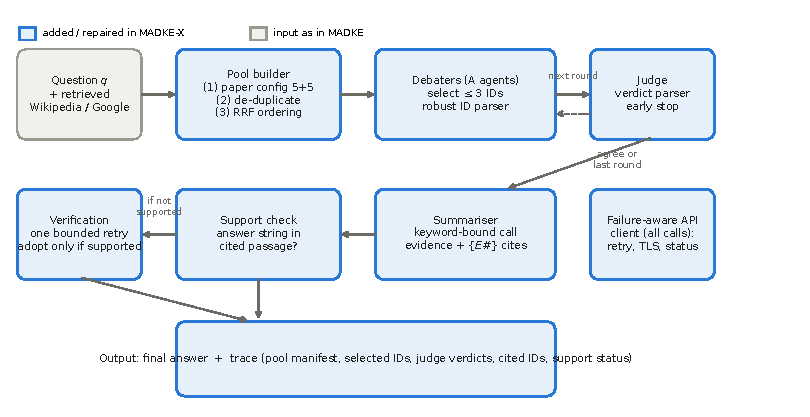
\includegraphics[width=\textwidth]{fig1_architecture}
\caption{MADKE-X architecture. Blue boxes are added or repaired relative to MADKE; the debate control flow is unchanged.}
\label{fig:architecture}
\end{figure}

\section{The proposed method: MADKE-X}
\label{sec:method}

\subsection{Failure-aware interface layer}
Every model call returns an explicit result (ok, error, attempts) from a client with bounded retries and verified TLS; a failed call marks the question as failed instead of letting an error message be scored as an answer. The summariser call is bound by keyword, evidence IDs are parsed by an order-preserving parser that keeps the first three IDs and records everything it ignores (Algorithm~\ref{alg:parse}), the judge verdict is the last bracketed Yes/No, case-insensitive, and the consistency statistics are computed from the stored judge texts including the final round.

\subsection{Evidence governor}
Algorithm~\ref{alg:pool} builds the pool. It uses the paper's configuration (5 Wikipedia + 5 Google passages), where the released code defaulted to 10 + 5, removes passages with identical normalised text, and orders the rest by reciprocal rank fusion of the retrieval rank and a question-only BM25 rank \cite{cormack2009rrf,robertson2009bm25}; no gold answer and no model is used.

\subsection{Decision trace and citations}
Each answer record carries a trace with (i) a pool manifest (index, source, source rank, passage hash), (ii) for every round and agent, the IDs actually delivered, with dropped, ignored and out-of-range IDs, (iii) the judge verdict and how it was parsed, and (iv) the final answer, the evidence IDs it cites as $\{E\#\}$ (a bracket type that cannot collide with the answer brackets) and the result of a support check (Algorithm~\ref{alg:support}). The check detects the \emph{absence} of the answer string from the cited passages; it does not establish entailment.

\begin{algorithm}[!htbp]
\caption{ParseEvidenceIDs}
\label{alg:parse}
\Input{reply $r$, pool size $m$, cap $k{=}3$}
\Output{IDs, not-found flag, audit lists}
$I \leftarrow [\,]$, $O \leftarrow [\,]$, $f \leftarrow \textbf{false}$\;
\ForEach{bracket group $g$ of $r$, in written order}{
  \lIf{$g$ matches no[\_ -]?found (any case)}{$f \leftarrow \textbf{true}$}
  \ElseIf{$g$ is a list of integers}{
    \ForEach{integer $n$ in $g$}{
      \lIf{$n \ge m$}{append $n$ to $O$}
      \lElseIf{$n \notin I$}{append $n$ to $I$}
    }
  }
}
\lIf{$f$}{\textbf{return} $([\,]$, \textbf{true}, ignored$=I$, dropped$=[\,]$, out-of-range$=O)$}
\textbf{return} $(I[{:}k]$, \textbf{false}, $[\,], I[k{:}], O)$\;
\end{algorithm}

\begin{algorithm}[!htbp]
\caption{BuildPool (evidence governor)}
\label{alg:pool}
\Input{question $q$, lists $W$ (Wikipedia), $G$ (Google), $w{=}5$, $g{=}5$, BM25 index $\mathcal{B}$}
\Output{ordered pool $E$}
$E \leftarrow W[{:}w] \,\|\, G[{:}g]$, recording source and source rank $\rho(e)$\;
remove $e$ whose normalised text was already seen\;
rank $E$ by $\mathrm{BM25}_{\mathcal{B}}(q,e)$ to obtain $\beta(e)$\;
\textbf{return} $E$ sorted by decreasing $\dfrac{1}{60+\rho(e)} + \dfrac{1}{60+\beta(e)}$\;
\end{algorithm}

\subsection{Bounded verification (new)}
When the status is not \emph{supported}, the summariser is called once more with the same evidence and an instruction to answer only if a listed passage states the answer, citing it, or otherwise to abstain with \texttt{[Unsupported] \{E-none\}}. The second answer is adopted only if its own support check passes; otherwise the first answer is kept and flagged in the trace. The step adds at most one call per question, never changes an answer that is already supported, and is switched off by default (\texttt{-verify}).

\begin{algorithm}[!htbp]
\caption{SupportCheck}
\label{alg:support}
\Input{answer $a$, cited IDs $C$, pool $E$}
\Output{status}
\lIf{$a = \varepsilon$}{\textbf{return} empty\_answer}
\lIf{$C = \emptyset$}{\textbf{return} no\_citation}
\lIf{normalised $a$ occurs in normalised text of some $E_i$, $i \in C$}{\textbf{return} supported}
\textbf{return} cited\_but\_answer\_not\_found\;
\end{algorithm}

\begin{algorithm}[!htbp]
\caption{MADKE-X (control flow)}
\label{alg:control}
\Input{question $q$, raw retrieval lists, $A$, $R$, flags cite and verify}
\Output{answer, trace}
$E \leftarrow$ BuildPool (Alg.~\ref{alg:pool})\;
\For{$r = 1$ \KwTo $R$}{
  \ForEach{debater $i$}{
    $(I_i) \leftarrow$ ParseEvidenceIDs(select($q$,$E$,$h_i$)) (Alg.~\ref{alg:parse}); $a_i \leftarrow$ answer($q$, $E[I_i]$, $h_i$)\;
  }
  $v \leftarrow$ ParseJudgeVerdict(judge($q$, $a_1..a_A$))\;
  \lIf{any call failed}{mark question failed; \textbf{break}}
  \If{$v = $ yes \textbf{or} $r = R$}{
    $s \leftarrow$ summarise($q$, $a_{1..A}$, $E[\cup I_i]$) with $\{E\#\}$ citations\;
    $c \leftarrow$ SupportCheck($s$)\;
    \If{verify \textbf{and} $c \neq$ supported}{
      $s' \leftarrow$ summarise with verification instruction; adopt $s'$ iff SupportCheck($s'$) $=$ supported\;
    }
    \textbf{break}\;
  }
}
\textbf{return} answer, trace\;
\end{algorithm}

\section{Complexity analysis}
\label{sec:complexity}

Let $A$ be the number of agents, $R$ the maximum number of rounds, $m$ the pool size, $L$ the mean passage length (words) and $N$ the number of passages in the BM25 reference set. Table~\ref{tab:complexity} compares the two systems analytically. The dominant cost of both systems is the LLM calls, whose number is unchanged except for the optional verification call. MADKE-X reduces the tokens in each selection call, and the number of such calls is $AR$ at most (6 at $A{=}2$, $R{=}3$).

\begin{table}[!htbp]
\centering
\small
\caption{Analytic cost of MADKE and MADKE-X per question.}
\label{tab:complexity}
\begin{tabular}{p{0.25\textwidth}p{0.29\textwidth}p{0.34\textwidth}}
\toprule
Quantity & MADKE & MADKE-X \\
\midrule
LLM calls (worst case) & $R(2A{+}1){+}1$ (16 at $A{=}2$, $R{=}3$) & $R(2A{+}1){+}1$, $+1$ with verification (17: $+6.25\%$) \\
Evidence listing per selection call & $(10{+}5)\cdot L$ words & $\le (5{+}5)\cdot L$ words ($-33\%$ passages) \\
Pool construction & $O(1)$ slice & $O(m\,|q|)$ after a one-time $O(NL)$ index \\
Auxiliary memory & none & $O(V)$ BM25 index, $V=$ vocabulary \\
Trace & none & $O(AR\cdot 3 + m)$ identifiers \\
\bottomrule
\end{tabular}
\end{table}

\section{Experimental design}
\label{sec:design}

The design reproduces that of MADKE so that the comparison is like for like (Table~\ref{tab:design}).

\paragraph{Component ablation} the steps are MADKE, then adding in turn the interface layer, the paper-sized pool, de-duplication, RRF ordering, citations and verification; each step is a separate run so that its effect is attributable.

\paragraph{Decision rule} The interface repairs are adopted if F1 does not drop beyond paired-bootstrap noise on any dataset; RRF and verification are adopted only if the pooled paired test is significant after Holm correction. A difference of 4.4 points near 50\% accuracy needs about 1,000 paired questions at an assumed agreement of 0.5 (Figure~\ref{fig:power}), so per-dataset results at $n{=}500$ are exploratory and the pooled analysis is primary.

\begin{table}[!htbp]
\centering
\small
\caption{Evaluation design: what MADKE did and what we do.}
\label{tab:design}
\begin{tabular}{p{0.14\textwidth}p{0.34\textwidth}p{0.40\textwidth}}
\toprule
 & MADKE (published) & This study \\
\midrule
Datasets & TriviaQA, NQ, HotpotQA, 2WikiMQA, FEVER, MMLU-Med; 500 each (595 MMLU-Med) & Same shipped files, unaltered, all 500 questions (the released code processes 441); MMLU-Med not shipped \\
Baselines & SP, CoT, SC, RAG, MAD & Same five, plus MADKE re-run and MADKE-X \\
Backbones & GPT-3.5-Turbo, Qwen1.5-32B/72B-Chat; GPT-4-Turbo reference & Same \\
Metrics & F1, GPT-4 score, EM (FEVER), Cons, Co2 & Same, with Cons/Co2 computed by the repaired metric; plus support status, failure count, tokens, time \\
Setting & Two agents, $\le$3 rounds, temperature 0.5, top-5 Wikipedia, 5 Google, $\le$3 items per round & Identical \\
Analyses & Knowledge-source ablation, selector ablation, model scale, agents/rounds, token cost, case study & Same, plus component ablation of MADKE-X \\
Statistics & Point estimates & Paired exact McNemar, paired bootstrap, Holm correction, pre-specified pooled analysis \\
\bottomrule
\end{tabular}
\end{table}

\subsection{Implementation and environment}
The code is Python \texttt{3.13.16} with the standard library for the debate loop and parsers; analyses use NumPy 2.5.3, SciPy 1.18.1 and Matplotlib 3.11.2; the manuscript is built with pdfTeX (TeX Live 2023). All offline experiments ran on a Linux 6.18 virtual machine with an Intel Xeon processor at 2.10\,GHz (two cores) and 8\,GB of memory. No GPU, LLM or search API was used. The scripted agents emit replies in the formats the prompts request, with deliberate format variation (lower-case flags, IDs in one bracket, quoted verdicts), so that each repaired parser is exercised against a known intended result.

\section{Results demonstrated offline}
\label{sec:offline}

\subsection{Data integrity}
The five shipped files are read-only; \texttt{sha256sum -c} reports all five unchanged after all experiments (checksums in Part~II).

\subsection{Correctness: MADKE-X versus MADKE}
On 160 questions per dataset, both systems ran under identical scripted agents (Figure~\ref{fig:invariants}, Tables~\ref{tab:invariants} and~\ref{tab:consistency}). MADKE gives the summariser the wrong prompt on all processed questions, delivers the evidence the agent chose for only 16\% of selections, stops at the wrong round for 22\%, and cannot credit agreement in the last round (Cons 67.7\% against a true 90.4\% on 3,000 synthetic debates); MADKE-X satisfies every invariant and reproduces the true consistency (90.4\%) and the true Co2 (54.2\%).

\begin{figure}[!htbp]
\centering
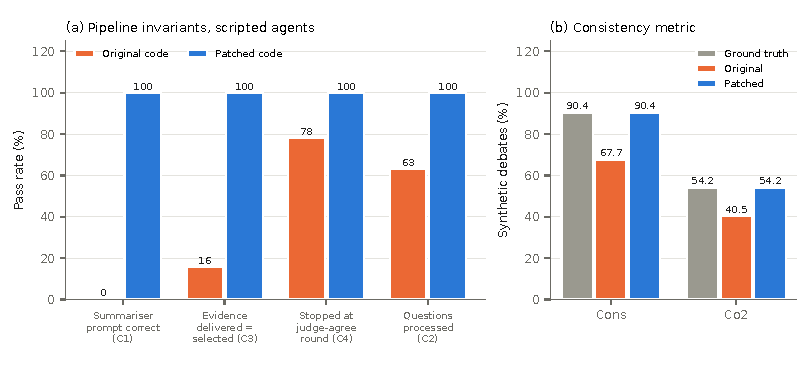
\includegraphics[width=\textwidth]{fig2_invariants_consistency}
\caption{(a) Invariant pass rates under scripted agents (TriviaQA; the scripted agents are index-based, so the rates are identical on all five datasets). (b) Consistency metrics against ground truth.}
\label{fig:invariants}
\end{figure}

\begin{table}[!htbp]
\centering
\small
\caption{Invariants, no injected failures (original = MADKE, patched = MADKE-X).}
\label{tab:invariants}
\resizebox{\textwidth}{!}{%
\begin{tabular}{lrrrrrrrr}
\toprule
 & \multicolumn{2}{c}{Processed} & \multicolumn{2}{c}{Summariser slot} & \multicolumn{2}{c}{Evidence delivered} & \multicolumn{2}{c}{Stop round} \\
\cmidrule(lr){2-3}\cmidrule(lr){4-5}\cmidrule(lr){6-7}\cmidrule(lr){8-9}
Dataset & Orig. & Patched & Orig. & Patched & Orig. & Patched & Orig. & Patched \\
\midrule
TriviaQA & 101 & 160 & 0\% & 100\% & 16\% & 100\% & 78\% & 100\% \\
NQ       & 101 & 160 & 0\% & 100\% & 16\% & 100\% & 78\% & 100\% \\
HotpotQA & 101 & 160 & 0\% & 100\% & 16\% & 100\% & 78\% & 100\% \\
2WikiMQA & 101 & 160 & 0\% & 100\% & 16\% & 100\% & 78\% & 100\% \\
FEVER    & 101 & 160 & 0\% & 100\% & 16\% & 100\% & 78\% & 100\% \\
\bottomrule
\end{tabular}%
}
\end{table}

\subsection{Evidence ordering}
Table~\ref{tab:ordering} and Figure~\ref{fig:ordering} show the share of questions with an answer-bearing passage among the first $k$; Table~\ref{tab:paired} gives the paired test. The ordering of MADKE (Wikipedia first) is below random on three of four sets, and RRF is above the random expectation on all four.

\begin{table}[!htbp]
\centering
\scriptsize
\caption{Consistency metrics against ground truth, with and without 3\% injected API failures.}
\label{tab:consistency}
\setlength{\tabcolsep}{3.5pt}
\resizebox{\textwidth}{!}{%
\begin{tabular}{llrrrrrrrrrr}
\toprule
 & & \multicolumn{4}{c}{Cons (\%)} & \multicolumn{4}{c}{Co2 (\%)} & \multicolumn{2}{c}{Failures} \\
\cmidrule(lr){3-6}\cmidrule(lr){7-10}\cmidrule(lr){11-12}
 & API & \multicolumn{2}{c}{Original} & \multicolumn{2}{c}{Patched} & \multicolumn{2}{c}{Original} & \multicolumn{2}{c}{Patched} & Scored & Flagged \\
\cmidrule(lr){3-4}\cmidrule(lr){5-6}\cmidrule(lr){7-8}\cmidrule(lr){9-10}
Dataset & fail & truth & metric & truth & metric & truth & metric & truth & metric & as text & (patched) \\
\midrule
TriviaQA & 0\% & 87.1 & 52.5 & 87.5 & 87.5 & 87.1 & 52.5 & 87.5 & 87.5 & 0 & 0 \\
TriviaQA & 3\% & 80.2 & 51.5 & 87.3 & 87.3 & 76.2 & 47.5 & 87.3 & 87.3 & 19 & 26 \\
NQ & 0\% & 87.1 & 52.5 & 87.5 & 87.5 & 87.1 & 52.5 & 87.5 & 87.5 & 0 & 0 \\
NQ & 3\% & 80.2 & 51.5 & 87.3 & 87.3 & 76.2 & 47.5 & 87.3 & 87.3 & 19 & 26 \\
HotpotQA & 0\% & 87.1 & 52.5 & 87.5 & 87.5 & 87.1 & 52.5 & 87.5 & 87.5 & 0 & 0 \\
HotpotQA & 3\% & 80.2 & 51.5 & 87.3 & 87.3 & 76.2 & 47.5 & 87.3 & 87.3 & 19 & 26 \\
2WikiMQA & 0\% & 87.1 & 52.5 & 87.5 & 87.5 & 87.1 & 52.5 & 87.5 & 87.5 & 0 & 0 \\
2WikiMQA & 3\% & 80.2 & 51.5 & 87.3 & 87.3 & 76.2 & 47.5 & 87.3 & 87.3 & 19 & 26 \\
FEVER & 0\% & 87.1 & 52.5 & 87.5 & 87.5 & 87.1 & 52.5 & 87.5 & 87.5 & 0 & 0 \\
FEVER & 3\% & 80.2 & 51.5 & 87.3 & 87.3 & 76.2 & 47.5 & 87.3 & 87.3 & 19 & 26 \\
\bottomrule
\end{tabular}%
}
\end{table}

\begin{figure}[!htbp]
\centering
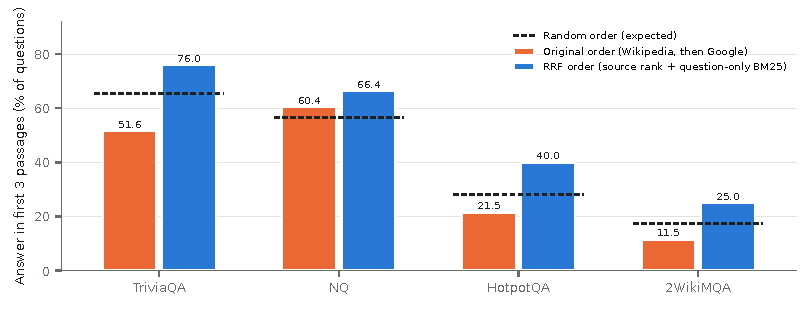
\includegraphics[width=\textwidth]{fig3_ordering}
\caption{Answer in the first three passages: MADKE order versus RRF order; the dashed line is the random-order expectation.}
\label{fig:ordering}
\end{figure}

\subsection{Cost: time, memory and tokens}
Table~\ref{tab:cost} and Figure~\ref{fig:cost} compare the two systems on all 500 questions of each dataset. The paper-sized pool reduces the evidence listing in every selection call by 44.8--45.3\% (mean 45.0\%; tokens estimated as characters/4, since no tokenizer was available); with at most six selection calls per question this is up to about 4,829 fewer input tokens per question on TriviaQA (4,841 on NQ), an upper bound because early stopping removes rounds. Ordering costs 0.68\,ms per question against 0.016\,ms for slicing, and peak memory is 6.9\,MB against 6.8\,MB. The parsers take 2.9 against 2.2 microseconds per call. These costs are negligible against the seconds a model call takes. We report no speed-up: in the zero-latency harness the per-question loop time (2.5\,ms for MADKE-X, 3.6\,ms with verification, 7.0\,ms for MADKE) is dominated by the harness matching questions in prompts, whose time grows with prompt length, and is therefore not a measure of system speed. The smaller pool is not free: it lowers the share of questions with any answer-bearing passage by 0.8 points (TriviaQA) to 3.4 points (NQ and HotpotQA) (Table~\ref{tab:poolcfg}).

\begin{table}[!htbp]
\centering
\small
\caption{Ordering on the shipped pools (percent of questions; MRR of the first answer-bearing passage).}
\label{tab:ordering}
\begin{tabular}{llrrrr}
\toprule
Dataset & Ordering & cov@1 & cov@3 & cov@5 & MRR \\
\midrule
\multirow{5}{*}{TriviaQA} & Original & 38.6 & 51.6 & 57.2 & 0.496 \\
 & Interleaved & 38.6 & 71.2 & 77.4 & 0.565 \\
 & BM25 & 53.6 & 75.0 & 79.0 & 0.646 \\
 & RRF & 55.2 & 76.0 & 79.2 & 0.657 \\
 & Random & 38.1 & 65.4 & 75.2 & 0.534 \\
\midrule
\multirow{5}{*}{NQ} & Original & 46.8 & 60.4 & 67.2 & 0.567 \\
 & Interleaved & 46.8 & 69.0 & 75.8 & 0.596 \\
 & BM25 & 35.4 & 62.8 & 73.0 & 0.513 \\
 & RRF & 44.2 & 66.4 & 75.0 & 0.571 \\
 & Random & 29.7 & 56.6 & 68.9 & 0.462 \\
\midrule
\multirow{5}{*}{HotpotQA} & Original & 15.9 & 21.5 & 24.9 & 0.225 \\
 & Interleaved & 15.9 & 33.5 & 39.4 & 0.269 \\
 & BM25 & 22.8 & 38.9 & 44.7 & 0.316 \\
 & RRF & 26.9 & 40.0 & 45.4 & 0.340 \\
 & Random & 12.9 & 28.2 & 36.7 & 0.228 \\
\midrule
\multirow{5}{*}{2WikiMQA} & Original & 6.4 & 11.5 & 15.0 & 0.126 \\
 & Interleaved & 6.4 & 21.6 & 28.6 & 0.165 \\
 & BM25 & 17.7 & 26.5 & 31.0 & 0.233 \\
 & RRF & 16.0 & 25.0 & 31.4 & 0.223 \\
 & Random & 7.0 & 17.4 & 25.1 & 0.148 \\
\bottomrule
\end{tabular}
\end{table}

\begin{table}[!htbp]
\centering
\small
\caption{Paired comparison, RRF versus MADKE order, cov@3.}
\label{tab:paired}
\setlength{\tabcolsep}{4pt}
\resizebox{\textwidth}{!}{%
\begin{tabular}{lrrrrcc}
\toprule
Dataset & $n$ & RRF only & Original only & Gain (pts) & 95\% bootstrap CI & Exact McNemar $p$ \\
\midrule
TriviaQA & 500 & 130 & 8 & $+24.4$ & [20.4, 28.4] & $1.6\times10^{-29}$ \\
NQ & 500 & 79 & 49 & $+6.0$ & [1.8, 10.6] & 0.010 \\
HotpotQA & 465 & 93 & 7 & $+18.5$ & [14.6, 22.4] & $2.7\times10^{-20}$ \\
2WikiMQA & 468 & 82 & 19 & $+13.5$ & [9.2, 17.7] & $1.7\times10^{-10}$ \\
\bottomrule
\end{tabular}%
}
\end{table}

\begin{table}[!htbp]
\centering
\small
\caption{Cost of MADKE (wiki 10 + Google 5, raw) and MADKE-X (paper pool, dedupe, RRF) on the shipped data.}
\label{tab:cost}
\setlength{\tabcolsep}{4pt}
\resizebox{\textwidth}{!}{%
\begin{tabular}{lrrrrrrr}
\toprule
 & \multicolumn{3}{c}{Evidence listing (est.\ tokens)} & \multicolumn{2}{c}{Pool build (ms/question)} & \multicolumn{2}{c}{Peak memory (MB)} \\
\cmidrule(lr){2-4}\cmidrule(lr){5-6}\cmidrule(lr){7-8}
Dataset & MADKE & MADKE-X & $-$\% & MADKE & MADKE-X & MADKE & MADKE-X \\
\midrule
TriviaQA & 1,778 & 973 & 45.3 & 0.014 & 0.646 & 7.0 & 6.5 \\
NQ & 1,801 & 994 & 44.8 & 0.017 & 0.598 & 6.7 & 6.2 \\
HotpotQA & 1,809 & 998 & 44.9 & 0.013 & 0.692 & 6.9 & 7.6 \\
2WikiMQA & 1,778 & 975 & 45.1 & 0.015 & 0.734 & 6.8 & 7.8 \\
FEVER & 1,793 & 987 & 45.0 & 0.020 & 0.709 & 6.8 & 6.3 \\
\bottomrule
\end{tabular}%
}
\end{table}

\begin{figure}[!htbp]
\centering
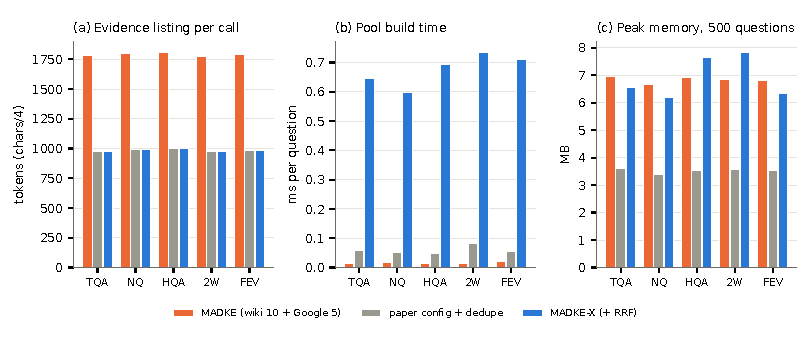
\includegraphics[width=\textwidth]{fig4_cost}
\caption{Evidence listing size, pool build time and peak memory over 500 questions per dataset.}
\label{fig:cost}
\end{figure}

\begin{table}[!htbp]
\centering
\small
\caption{Pool configurations (coverage = questions with an answer-bearing passage).}
\label{tab:poolcfg}
\setlength{\tabcolsep}{4pt}
\resizebox{\textwidth}{!}{%
\begin{tabular}{llrrrr}
\toprule
Dataset & Pool configuration & Passages & Words & Coverage (\%) & Dupes removed \\
\midrule
\multirow{3}{*}{TriviaQA} & code default (wiki 10 + Google 5) & 14.54 & 1,142 & 83.2 & 0 \\
 & paper (wiki 5 + Google 5) & 9.54 & 628 & 82.4 & 0 \\
 & patched (wiki 5 + Google 5, de-duplicated) & 9.52 & 626 & 82.4 & 10 \\
\midrule
\multirow{3}{*}{NQ} & code default (wiki 10 + Google 5) & 14.99 & 1,159 & 86.4 & 0 \\
 & paper (wiki 5 + Google 5) & 9.99 & 643 & 83.0 & 0 \\
 & patched (wiki 5 + Google 5, de-duplicated) & 9.98 & 641 & 83.0 & 7 \\
\midrule
\multirow{3}{*}{HotpotQA} & code default (wiki 10 + Google 5) & 14.94 & 1,148 & 50.5 & 0 \\
 & paper (wiki 5 + Google 5) & 9.94 & 634 & 47.1 & 0 \\
 & patched (wiki 5 + Google 5, de-duplicated) & 9.93 & 633 & 47.1 & 7 \\
\midrule
\multirow{3}{*}{2WikiMQA} & code default (wiki 10 + Google 5) & 14.80 & 1,146 & 40.4 & 0 \\
 & paper (wiki 5 + Google 5) & 9.80 & 631 & 37.4 & 0 \\
 & patched (wiki 5 + Google 5, de-duplicated) & 9.78 & 629 & 37.4 & 9 \\
\bottomrule
\end{tabular}%
}
\end{table}

\subsection{Trace and verification (structure only)}
Over 800 scripted debates every trace matches the evidence actually delivered (320/320 selections per dataset), every citation resolves to the pool and to a selected passage, and adding citations never changes the final answer. Table~\ref{tab:verification} and Figure~\ref{fig:verification} show the verification step on scripted agents whose summariser first cites an arbitrary selected passage: verification is triggered only for unsupported answers, is adopted only when the retry is supported, and increases the number of supported answers (for example 29 to 44 of 160 on NQ). Because the scripts are not models, these counts illustrate that the mechanism works, not how often a real model would be helped.

\begin{table}[!htbp]
\centering
\small
\caption{Verification on scripted agents (160 questions per dataset).}
\label{tab:verification}
\setlength{\tabcolsep}{4pt}
\resizebox{\textwidth}{!}{%
\begin{tabular}{lrrrrrrr}
\toprule
 & \multicolumn{3}{c}{Citations only (of 160)} & \multicolumn{4}{c}{Citations + verification} \\
\cmidrule(lr){2-4}\cmidrule(lr){5-8}
Dataset & supported & not found & no citation & supported & retries & adopted & answers changed \\
\midrule
TriviaQA & 10 & 98 & 52 & 13 & 150 & 3 & 0 \\
NQ & 29 & 79 & 52 & 44 & 131 & 15 & 0 \\
HotpotQA & 13 & 95 & 52 & 31 & 147 & 18 & 0 \\
2WikiMQA & 3 & 105 & 52 & 11 & 157 & 8 & 0 \\
FEVER & 0 & 108 & 52 & 1 & 160 & 1 & 0 \\
\bottomrule
\end{tabular}%
}
\end{table}

\begin{figure}[!htbp]
\centering
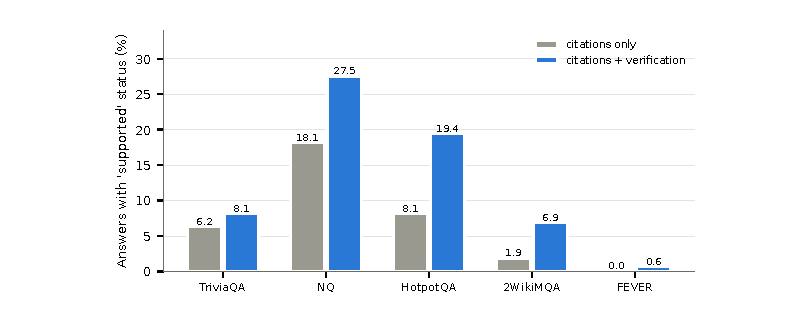
\includegraphics[width=\textwidth]{fig5_verification}
\caption{Supported answers with and without verification (scripted agents).}
\label{fig:verification}
\end{figure}

\section{End-to-end comparison (accuracy pending)}
\label{sec:live}

Table~\ref{tab:main} is laid out like Table~2 of MADKE \cite{wang2025madke}. Published values are transcribed from that paper (arXiv v2) and are not re-measured; the cells marked ``--'' are empty because no model was available. They are not estimates, and nothing in this paper should be read as a prediction of them. The ``re-run'' row is needed because a published number and a number from our harness can differ in prompts, sampling and judge.

\begin{table}[!htbp]
\centering
\tiny
\caption{Main comparison protocol. F1 and GPT-4 score (G4) for generative QA, exact match for FEVER. Rows other than the two marked ones are transcribed from the base paper; ``--'' = not yet measured.}
\label{tab:main}
\setlength{\tabcolsep}{3.2pt}
\resizebox{\textwidth}{!}{%
\begin{tabular}{llccccccccc}
\toprule
Backbone & Method & TQA F1 & TQA G4 & NQ F1 & NQ G4 & HQA F1 & HQA G4 & 2W F1 & 2W G4 & FEV EM \\
\midrule
\multirow{8}{*}{GPT-3.5-Turbo}
 & SP & 0.761 & 0.778 & 0.390 & 0.532 & 0.331 & 0.384 & 0.190 & 0.210 & 0.548 \\
 & CoT & 0.715 & 0.772 & 0.418 & 0.588 & 0.333 & 0.410 & 0.165 & 0.190 & 0.556 \\
 & SC & 0.756 & 0.818 & 0.431 & 0.622 & 0.342 & 0.408 & 0.175 & 0.206 & 0.560 \\
 & RAG & 0.768 & 0.824 & 0.450 & 0.436 & 0.423 & 0.498 & 0.204 & 0.228 & 0.646 \\
 & MAD & 0.712 & 0.798 & 0.401 & 0.648 & 0.287 & 0.394 & 0.133 & 0.186 & 0.548 \\
 & MADKE (as published) & 0.728 & 0.830 & 0.453 & 0.736 & 0.405 & 0.542 & 0.205 & 0.274 & 0.612 \\
 & MADKE (re-run, our harness) & -- & -- & -- & -- & -- & -- & -- & -- & -- \\
 & \textbf{MADKE-X (ours)} & -- & -- & -- & -- & -- & -- & -- & -- & -- \\
\midrule
\multirow{8}{*}{Qwen1.5-32B-Chat}
 & SP & 0.581 & 0.632 & 0.295 & 0.462 & 0.311 & 0.384 & 0.207 & 0.220 & 0.536 \\
 & CoT & 0.587 & 0.644 & 0.276 & 0.452 & 0.315 & 0.382 & 0.220 & 0.228 & 0.546 \\
 & SC & 0.583 & 0.628 & 0.276 & 0.442 & 0.312 & 0.386 & 0.203 & 0.222 & 0.540 \\
 & RAG & 0.446 & 0.554 & 0.269 & 0.436 & 0.309 & 0.420 & 0.183 & 0.248 & 0.664 \\
 & MAD & 0.630 & 0.704 & 0.321 & 0.566 & 0.363 & 0.482 & 0.256 & 0.286 & 0.520 \\
 & MADKE (as published) & 0.763 & 0.838 & 0.475 & 0.724 & 0.450 & 0.570 & 0.258 & 0.314 & 0.646 \\
 & MADKE (re-run, our harness) & -- & -- & -- & -- & -- & -- & -- & -- & -- \\
 & \textbf{MADKE-X (ours)} & -- & -- & -- & -- & -- & -- & -- & -- & -- \\
\midrule
\multirow{8}{*}{Qwen1.5-72B-Chat}
 & SP & 0.665 & 0.706 & 0.378 & 0.550 & 0.332 & 0.428 & 0.226 & 0.260 & 0.596 \\
 & CoT & 0.715 & 0.776 & 0.406 & 0.648 & 0.431 & 0.514 & 0.275 & 0.324 & 0.625 \\
 & SC & 0.659 & 0.700 & 0.369 & 0.548 & 0.336 & 0.430 & 0.207 & 0.242 & 0.596 \\
 & RAG & 0.662 & 0.762 & 0.333 & 0.710 & 0.438 & 0.538 & 0.217 & 0.304 & 0.668 \\
 & MAD & 0.703 & 0.796 & 0.376 & 0.660 & 0.397 & 0.548 & 0.274 & 0.344 & 0.516 \\
 & MADKE (as published) & 0.787 & 0.874 & 0.479 & 0.748 & 0.495 & 0.622 & 0.284 & 0.350 & 0.686 \\
 & MADKE (re-run, our harness) & -- & -- & -- & -- & -- & -- & -- & -- & -- \\
 & \textbf{MADKE-X (ours)} & -- & -- & -- & -- & -- & -- & -- & -- & -- \\
\midrule
GPT-4-Turbo & SP (reference) & 0.828 & 0.902 & 0.459 & 0.692 & 0.472 & 0.566 & 0.265 & 0.284 & 0.608 \\
\bottomrule
\end{tabular}%
}
\end{table}

\paragraph{Planned additional analyses} (i) Knowledge source (none, Wikipedia, Google, both) with and without the evidence governor; (ii) component ablation (Section~\ref{sec:design}); (iii) model scale (Qwen1.5 1.8B--72B); (iv) number of agents and rounds on GPT-3.5-Turbo; (v) token cost against MADKE and MAD, where the published MADKE figure is 27.5\% fewer output tokens than MAD; (vi) consistent-but-wrong rate and support-status distribution, which only MADKE-X can report; (vii) a case study with a printed trace; and (viii) a human audit of 100 answers for GPT-4-score agreement.

\begin{figure}[!htbp]
\centering
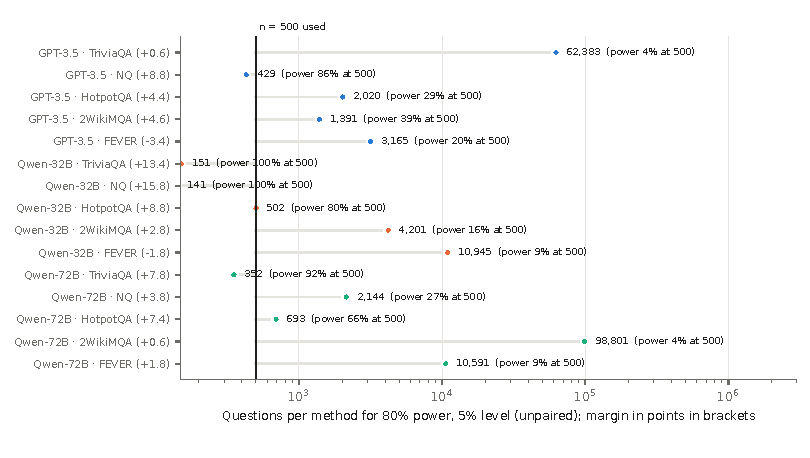
\includegraphics[width=\textwidth]{fig6_power}
\caption{Questions needed for 80\% power at each published margin; the line marks $n{=}500$. Differences below roughly 5 points are not resolvable per dataset at this size.}
\label{fig:power}
\end{figure}

\section{Discussion}
\label{sec:discussion}

\paragraph{Where MADKE-X is better, and where this is shown.} MADKE-X is better than MADKE in correctness (every tested invariant), in evidence ordering (answer-bearing passages come earlier, with paired significance), in per-call input size (about 45\% smaller listing, estimated), in completeness (all 500 questions, failures flagged not scored) and in explainability (a trace and a support check for every answer). It is slower only by the order of a millisecond per question, and uses the same memory.

\paragraph{Where this is not shown} We do not show that MADKE-X answers more questions correctly. The ordering gain is a property of the evidence, models may use the pool differently from our counts, and the smaller pool lowers the coverage ceiling slightly. Document-level retrieval failures remain: only 50.5\% (HotpotQA) and 40.4\% (2WikiMQA) of questions have any answer-bearing passage at all. A label-free pool-sufficiency gate did not work (AUC 0.475--0.616) and is not part of MADKE-X. The support check is lexical, so it can mark a correct paraphrase as unsupported and a coincidental string as supported.

\paragraph{Practical value} For a deployed question-answering system, traceability and bounded failure handling matter independently of accuracy: they make every answer inspectable, make failures countable, and make comparisons between configurations reproducible.

\section{Threats to validity}
\label{sec:threats}

(1) Scripted agents test formats, not reasoning. (2) Coverage uses a string match with the gold answer. (3) Token counts are estimated from characters. (4) Published baseline numbers are transcribed from a paper whose own tables contain inconsistencies reported earlier; the implied sample size fits $n{=}500$ rather than 441. (5) Reference metadata was checked for existence, venue and year, not author lists or page ranges. (6) The verification step was designed after the audit and has no model evidence.

\section{Conclusion}
\label{sec:conclusion}

MADKE-X keeps the debate design of MADKE and removes the implementation defects that undermine it, orders the evidence in a way that measurably brings answer-bearing passages forward, shrinks each selection prompt by about 45\%, and records a trace and a support check for every answer with an optional verification step. These claims are demonstrated offline on the unaltered shipped data. The accuracy comparison is specified in full and awaits model access; Table~\ref{tab:main} is where it will be reported.

\section*{CRediT authorship contribution statement}
Roles to be confirmed by the authors before submission.

\section*{Declaration of competing interest}
The authors declare no competing interests.

\section*{Declaration of generative AI and AI-assisted technologies in the writing process}
During the preparation of this work the authors used Claude (Anthropic) to assist with code, analysis scripts and drafting. The authors reviewed and edited the content and take full responsibility for the publication.

\section*{Data and code availability}
The patched code, patch, scripts, JSON outputs and data checksums accompany this manuscript. The datasets are those distributed with the MADKE repository (commit 9cd57ca) and are used unmodified.


\bibliographystyle{elsarticle-num}
\bibliography{references}

\end{document}
